\documentclass{article}
\usepackage{filecontents}
\usepackage[left=2.5cm,top=2.5cm,right=2.5cm,bottom=2.5cm]{geometry}
\usepackage{amsmath}
\usepackage{array}
\usepackage{caption}
\usepackage{placeins}
\usepackage[colorlinks=true,citecolor=blue]{hyperref}
\usepackage{graphicx}
\usepackage{subcaption}
\usepackage{setspace}
\usepackage{natbib}
\usepackage{rotating}
\usepackage{pdflscape}
\bibpunct{(}{)}{,}{a}{}{;}
\usepackage{url}
\usepackage{nth}
\usepackage{authblk}
\usepackage{multirow}
\usepackage{listings}
% for the d in integrals
\newcommand{\dd}{\; \mathrm{d}}
\newcommand{\tc}{\quad\quad\text{,}}
\newcommand{\tp}{\quad\quad\text{.}}
\bibliographystyle{apalike}
\usepackage[table]{xcolor} 

\title{Lifespan dispersion in times of life expectancy fluctuation: the case of Central and Eastern Europe}

\author[]{Authors Redacted}
\date{}
\begin{document}


\maketitle

\begin{abstract}
Central and Eastern Europe have experienced considerable instability in mortality since the 1960s. Long periods of stagnating life expectancy were followed by rapid increases in life expectancy and in some cases even more rapid declines before more recent periods of improvement. These trends have been well documented but to date, no study has comprehensively explored trends in lifespan variation.  We improve such analyses by incorporating life disparity as a health indicator alongside life expectancy. We analyzed how lifespan variation has changed since the 1960s for 12 countries from the region and determined the ages which have contributed the most to the observed variability in age at death. Furthermore, we quantified the effect of mortality related to alcohol consumption on life disparity since 1994. Our results showed that life disparity was high and strongly fluctuating over the time period. Life expectancy and life disparity moved independently from one another, particularly during periods of life expectancy stagnation. Fluctuations in mortality were, to a large extent, directly or partially attributable to changes in alcohol consumption. These trends run counter to the common patterns observed in most developed countries and contribute to the life expectancy-disparity discussion by showing that expansion/compression levels do not necessarily mean lower/higher life expectancy or mortality deterioration/improvements. 
\end{abstract}


\newpage

\begin{spacing}{1.5}
\section*{Introduction}
The \nth{20} century was marked by sizable improvements in mortality and health in most countries in the world \citep{who2000}. However, these improvements were unevenly shared in the second half of the past century, as parts of Central and Eastern Europe experienced an unprecedented period of stagnation and, in some countries, decrease in life expectancy at birth after 1960 \citep{HMD}. The long term combination of a failure to complete the epidemiologic transition by reducing cardiovascular diseases \citep{caselli2002epidemiologic}, along with fluctuation in alcohol and violence \citep{bye2008alcohol,leon1997huge}, led to lower levels of life expectancy and larger mortality inequalities in this region compared with western countries in Europe \citep{mackenbach2008socioeconomic}. The high mortality among young men is at the heart of Eastern European trends in life expectancy \citep{mckee2001}. For example, male life expectancy stagnated at a level between 65 and 70 years from the 1960s to the mid-1980s in Belarus, Bulgaria, Czech Republic, Estonia, Hungary, Latvia, Lithuania, Poland, Slovakia, Slovenia and Ukraine. During this same period, Russia experienced the lowest male life expectancy in the region, followed by a brief period of sizable improvements in life expectancy due to Gorbachev's anti-alcohol campaign \citep{leon1998social}. After 1987 the mortality experiences in the region diverged. Life expectancy increased continuously in Slovenia and the Czech Republic. The rest of the countries, particularly those from the former Soviet Union, experienced a pronounced period of deterioration up to the mid-1990s. Mortality increases among Russian and Latvian men were especially sharp, with life expectancy losses of around 7.5 years between 1987 and 1994, which led to levels not seen since the 1950s \citep{shkolnikov2001}. Since the mid-1990s, life expectancy has mostly been increasing throughout the region, but at different rates. As a result, large regional differences in survival have emerged. For instance, the 2010 gap in male life expectancy between Slovenia and Russia was more than 13 years \citep{HMD}.\\

National trends in life expectancy are important and have been extensively studied in the region \citep{mesle2004mortality, mesle2000, rychtarikova2004case,shkolnikov2001,shkolnikov2006changing,leon2011}. Nonetheless, as an average, life expectancy conceals considerable heterogeneity in individual mortality trajectories \citep{edwards2005, wilmoth1999}. This age-at-death variation, hereafter referred to as life disparity or lifespan variation, is an important dimension of inequality as it summarizes the uncertainty in the timing of death. Until now, trends in lifespan variation have mostly been studied in the context of mortality decline at all ages \citep{edwards2005,smits2009,vaupel2011}. Alongside increases in life expectancy, ages at death have become more predictable (i.e. lifespan variation has decreased). This is because mortality decline over young ages has outpaced mortality decline at older ages, compressing most deaths into a narrower age window \citep{vaupel2011}.\\

This need not be the case. At the subpopulation level, numerous instances have been documented of lifespan variation increase occurring alongside increases in life expectancy \citep{vanraalte2014,sasson2016trends,seaman2016increasing, bronnum-hansen2017}, mainly due to stalls in working age mortality decline occurring alongside continued old age mortality decline. To date, no comprehensive studies of lifespan variation have been undertaken under periods of life expectancy decline.\\

We complement the existing literature by focusing on the Central and Eastern European case, which shows atypical periods of mortality upheaval and substantial life expectancy fluctuation. This region is particularly interesting because its age pattern of mortality change was very different from that observed in western countries \citep{mesle2004mortality}. Since the sharpest fluctuation in age-specific mortality occurred over working ages \citep{rehm2007}, it is a priori unclear what the net effect would be on variability. We analyzed how lifespan variation has changed since the 1960s for 12 countries from this region and determined the ages and causes of death that contributed the most to the observed change in lifespan variation, with a particular focus on the impact of alcohol-attributable mortality. \\

Our analyses revealed three important findings: (1) the acute mortality crises of the 1990s caused greater year-to-year fluctuation in lifespan variation than in life expectancy, (2) life expectancy and lifespan variation moved independently, particularly during periods of stagnation and uneven age-specific mortality change, and (3) mortality amenable to alcohol consumption occurred over ages that both increased and decreased lifespan variation, with different net effects depending on the country and time period. These results underscore the added value of looking at other summary measures of mortality beyond the mean.


\section*{Data \& Methods}

\subsection*{Dispersion measure \& demographic methods}

For each population, we investigated life expectancy and lifespan variation since birth. We decided not to analyze variability at death conditioned on survival to a childhood age, as previous studies have done (e.g. \citet{edwards2005, smits2009}), because of the arbitrariness of choosing a starting age and because infancy and childhood are major contributors to lifespan inequalities that we did not want to overlook. 
Several dispersion measures have been proposed to analyze lifespan variability \citep{vanraalte2013, wilmoth1999}. In this article, we use life disparity ($e^{\dagger}$ ) as a dispersion indicator \citep{vaupel&Canudas2003}. It is defined as the average remaining life expectancy when death occurs; or life years lost due to death.  For example, when death is highly variable, some people will die well before their expected age at death, contributing many lost years to life disparity. When survival is highly concentrated around older ages, the difference between the age at death and the expected remaining years decreases, and life disparity gets smaller.  It can be expressed as
\begin{equation}
\label{eq.edagger}
e_x^{\dagger}=\frac{1}{\ell_x}\int_x^\omega \ell(a) \mu(a)e(a)da
\end{equation}
where $\ell(a)$, $\mu(a)$ , $\omega$ and $e(a)$ are the survival function, the force of mortality, the open-aged interval (110+ in our case), and remaining life expectancy, respectively. 
We selected this measure because of its easy public health interpretation, which equals the average life expectancy losses attributable to death \citep{shkolnikov2011}, and its decomposable and additive properties \citep{zhang2009}. The $e^\dagger$ measure has the additive property that, once it has been decomposed by age between two periods, the sum of every age-specific contribution to the difference is the total change in $e^\dagger$ between these two periods. These properties allow us to quantify the impact of mortality at different ages, and from different causes, and to separate ages that decrease lifespan variability from those that increase it by using demographic methods \citep{zhang2009, shkolnikov2011}. We perform such decomposition by single age, period and cause of death based on a continuous change model \citep{horiuchi2008} that has the advantage of assuming that covariates change gradually along the time dimension, for the age-cause decomposition we used the 5-year age group mortality rates from the \cite{HcO}. All the calculations were performed using \textit{R} \citep{team2000r} and are fully reproducible with the available \href{}{code and additional information}\footnote{Link to code removed to avoid identifying information}.\\

 
The close relationship with other lifespan variation indices, such as Keyfitz's life table entropy \citep{vaupel&Canudas2003}, and the high correlation between them suggests that conclusions would likely be the same regardless of the measure chosen \citep{vanraalte2013,vaupel2011,wilmoth1999}.\\


\subsection*{Data}
We used all-cause death counts, population exposures and period life tables from the \citet{HMD} for 12 countries from 1960 to the most recent year available in the data set. The countries included in the study were Belarus, Bulgaria, Czech Republic, Hungary, Poland, Russia, Slovakia, Ukraine, Slovenia, Estonia, Latvia and Lithuania. Data for Slovenia was only available from 1983. The data are by single age, year, sex and country.\\

Cause of death data came from the newly developed \citet{HcO}, which provides coherent cause-specific mortality data time series for eight of the countries in the study (Belarus, Czech Republic, Poland, Russia, Ukraine, Slovenia, Estonia, Latvia and Lithuania). For inclusion into the database, a universal and standardized methodology was undertaken to redistribute deaths between 104 disease categories in 5-year age groups. We used these data to get the cause-specific proportion by 5-year age groups. This has effectively eliminated ruptures surrounding revisions of the International Classifications of Disease (ICD), and substantially reduced cross-country comparability problems owing to different coding practices, particularly from the use of ill-defined and unknown causes. We truncated the cause-of-death analysis at age 85 because of classification quality and presence of comorbidities and focus on the period after 1994 because comparable information is available for the eight countries \citep{HcO}. Furthermore, we focus on this period because it coincides with the beginning of the divergence in Eastern European mortality trends, particularly between the former Soviet and Central European countries \citep{mesle2004mortality}.\\

\emph{Cause of death classification}\\

Injurious alcohol consumption has long been identified as a major determinant of premature mortality in Eastern European countries \citep{leon1997huge,mckee2001,rehm2007,grigoriev2015}. We aimed to identify the effect of mortality related to alcohol consumption on lifespan variation from 1994 to 2010. \\

We grouped causes of death into four categories according to the degree to which they associate with alcohol consumption and abuse (for details on the ICD-10 codes for each cause, see Table \ref{T1}). The categories are as follows:
1) Alcohol-attributable conditions (for example, mental and behavioral disorders due to use of alcohol, alcohol liver disease, accidental poisoning by alcohol); 2) Conditions amenable to alcohol consumption (such as ischemic heart disease (IHD), stroke and transportation accidents); 3) Other conditions susceptible to alcohol consumption (other external causes and other circulatory conditions); and 4) all other causes (labeled as residual causes). 
The first category (alcohol-attributable conditions) refers to those health conditions that by the ICD definition identifies alcohol consumption as a necessary cause and that previous research has identified as wholly attributable to alcohol consumption \citep{rehm2010relation}. We additionally include liver cirrhosis in this first category because around three-quarters of deaths from this cause in the region are thought to be attributable to alcohol \citep{rehm2003relationship}, and it is common practice to include it as a condition attributable to alcohol consumption \citep{rehm2003relationship,rehm2010relation}. \\
	
The second category, conditions amenable to alcohol consumption, pertains to conditions that are not wholly attributable to alcohol consumption, but that have been linked with alcohol consumption patterns. For example, heavy drinking is associated with physiological mechanisms that increase the risk of IHD and stroke death \citep{rehm2010relation}.  Similarly, alcohol consumption has been shown to have a causal impact on different injuries \citep{rehm2003relationship}. We focus on transport injuries because Latvia,
Lithuania and Russian report the highest in Europe \citep{avenoso2005safety} and recent developments in infrastructure and safety may have had an important impact in reducing transportation injuries in some countries \citep{world2009european,world2013global}. From this group of causes we are more interested in examining changing trends, which we expect to be more closely related to changing alcohol consumption patterns than the baseline levels, which have numerous determinants. \\

The third category, other conditions susceptible to alcohol consumption, includes the rest of external causes, such as self-inflicted injuries, and the rest of circulatory diseases. We analyze them separately to complement the broad categories of external and circulatory disease included in the second category. Although additional rare causes of death can be linked to alcohol consumption, we do not include them in our study because their absolute contributions to mortality change are likely to be very small in the set of countries that we study \citep{grigoriev2015}.


\begin{center}
[Table \ref{T1} about here]
\end{center}



In what follows, we present our results on Eastern European males only. Mortality fluctuated more strongly among men, which more clearly illustrates the added value of looking to lifespan variation in times of crisis. In most cases, trends were similar for both sexes, but the magnitude of change was less for females. Full results are presented in the supplemental material for females.



\section*{Results}
\emph{Age-specific mortality rates of improvements}\\

For a descriptive look at age-specific mortality change over the period, we first examined the average annual rate of mortality improvement \citep{Rau2013} with smoothed mortality surfaces \citep{Camarda2012} for males in 12 Central and Eastern European countries \ref{Fig_ROMI}. The respective values are expressed in percent. Little change or no improvement (-0.5\% to 0.5\%) is depicted in white. Improvement in mortality (i.e. mortality decline) is shown in blue and mortality increase in red. Darker tones mean major changes in mortality rates.\\

Almost every country experienced a near-continuous 20-year period of increasing mortality rates, from the mid-1960s to the mid-1980s. Mortality rate increases were mainly concentrated in the ages between 20 and 80 years. After 1985, 7 countries experienced sizable reductions in mortality rates (Belarus, Estonia, Latvia, Lithuania, Poland, Russia and Ukraine) for a period of around 5 years. Opposing this trend, in the early 1990s most countries that were part of the former Soviet Union such as Estonia, Latvia, Lithuania, Russia and Ukraine experienced intense mortality increases. Finally, since the mid to late 1990s Slovakia, Slovenia, Hungary, Latvia, Poland, Estonia and Czech Republic have reduced age-specific mortality rates at almost every age. The biggest improvements were related to the most recent years.\\



\begin{center}
[Figure \ref{Fig_ROMI} about here]
\end{center}

\emph{Trends in life expectancy and lifespan disparity}\\

Figure \ref{Fig_LE&LD} shows male $e_0$ and $e^{\dagger}$ trends for Central and Eastern European countries from 1960 to the most recent year available. From 1960 to 1984 $e_0$ stagnated for most of the countries, some of them even experienced a slow and steady decline (e.g. Russia, Latvia, Estonia, and Ukraine). This period was followed by a notable increase in $e_0$ in the mid-1980s, closely corresponding to, although sometimes preceding, Gorbachev's anti-alcohol campaign shaded in red. However, after 1987 life expectancy among these countries started to diverge: Central European countries experienced a short period of stagnation or decline followed by an upward trend until the end of the study. Russia, Latvia, Estonia, Ukraine, Belarus and Lithuania experienced a marked decrease in $e_0$ from 1988 to 1994. From that point on, $e_0$ improved everywhere, with the exception of Russia, Belarus and Ukraine. These last countries exhibited a final decrease (Russia) or stagnation (Belarus, Ukraine) in life expectancy between 1998 and the mid-2000s, followed by sharp increases in the final period from the mid-2000s to the latest available year. Importantly, Estonia shows exceptional improvements since the mid 1990's, particularly in women. \\

Life disparity showed similar patterns of stagnation between 1960 and 1980 as was seen for $e_0$. Russia and Lithuania exhibited the highest levels in this period, between 17 and 19 years lost due to death; while the Czech Republic presented the lowest level throughout the same years, between 13 and 14 years. Importantly, the Czech Republic was not the regional record $e_0$ holder during these years. Around the mid-1980s all countries experienced compression of mortality, i.e. decreases in $e^{\dagger}$, with the exception of Hungary. After 1991, Lithuania, Russia, Latvia and Estonia experienced significant increases in $e^{\dagger}$ with the peak in 1994-1995. During this peak, the observed $e_0$ levels differed from historic levels observed when $e^{\dagger}$ was equally high. Central European countries experienced continuous reductions in $e^{\dagger}$ after 1994, whereas it was less systematic in Latvia and Lithuania. The rest of the countries also experienced declines after that year up to 2010-2014, but with greater fluctuation. Such declines, however, were not as steep as the $e_0$ increases in these countries.\\
 
\begin{center}
[Figure \ref{Fig_LE&LD} about here]
\end{center}

\emph{Absolute and relative changes in life expectancy and lifespan disparity}\\

Contrasting the changing levels of $e_0$ and $e^\dagger$ from Figure \ref{Fig_LE&LD} suggests that in periods of stagnation and mortality upheavals  similar levels of $e_0$ do not correspond to similar levels in $e^\dagger$. Therefore, we analyzed the direction and magnitude of change in the two measures. \\

Figure \ref{Abs_changes} shows absolute and relative yearly changes (first differences) in $e_0$ and $e^\dagger$ by sex and period. If a negative relationship exists between $e_0$ and $e^\dagger$, changes would concentrate in the top left and bottom right quadrants. If points fall in the top right and bottom left quadrants, the relationship is positive. We focus on the latter changes and quantify their frequency in three different time periods relating to overall mortality trends. The period 1960-1987 contains a mixture of stagnation, steady decline and improvements in life expectancy; 1988 to 1995 was a period of decreasing life expectancy; and 1996 onwards is characterized by divergence between countries in life expectancy trends, with recent life expectancy improvements. Grey dots correspond to a negative association between life expectancy and life disparity (e.g. increases in $e_0$ with decreases in $e^\dagger$ ), while red dots correspond to a positive association (e.g. increases in $e_0$with increases in $e^\dagger$ ). Since Russia is both the largest country included in the analysis and the country with the most volatile mortality trends, we marked its points in dark blue. Absolute changes (top panel) are easy to interpret since they reflect the changes in life expectancy and life disparity measured in years. However, since the maximum value of $e_0$ is much higher than the maximum value of $e^\dagger$, it is not surprising that changes vary more strongly on the  $e_0$ axis than the $e^\dagger$ axis. Therefore, it is also important to analyze changes in both measures in relative terms (bottom panel).  This allows us to quantify the intensity of such changes.\\

During 1960-1987, almost one-third of the yearly changes in mortality resulted in $e_0$ decreases and decreases in $e^\dagger$, in both males (33.2\%, 95\% CI [27.9,38.5] ) and females (32.6 [27.3,37.9]). These were mostly small changes corresponding to less than one year of life. Conversely, 20.9\% [16.3,25.5] (males) and 25.9\% [21,30.9](females) of $e_0$ increases corresponded to $e^\dagger$ increase. This means that, by adding both quadrants, the measures in this period were moving in the same direction more than half of the time.  In 1988-1995, when most of the changes corresponded to substantial decreases in $e_0$, the two indices moved in the same direction about a quarter of the time. Finally in the period 1996 onwards, characterized by mortality convergence, more than a third of all points related to movements in the same direction for both measures. \\

Moreover, even when the two measures moved in the direction expected from a negative correlation, the magnitude of change in life expectancy did not reflect the same magnitude of change in life disparity. For example, Russia lost 3 years of male life expectancy (around 5\%) between 1992 and 1993, while life disparity showed a much smaller increase (less than 2.5\%). Most of the time, however, $e^\dagger$ experienced larger relative changes than $e_0$, evidenced by more movement along the horizontal than the vertical axis in the bottom panel of Figure \ref{Abs_changes}.


\begin{center}
[Figure \ref{Abs_changes} about here]
\end{center}

\emph{Age-specific decomposition}\\



Figure  \ref{MalesDecomp} shows age-specific contributions to the change in $e^\dagger$ for ages 5 and above\footnote{For age-specific contributions to life expectancy, see the supplemental material.}, respectively, by period (results for ages 0-4 depicted in Supplemental material Figure 7\footnote{Declines in mortality below age 5 were the strongest age-category contributor to changes in life disparity over the period under study, with most of the decline occurring over the 1960-1980 period. For this reason they are plotted separately from other ages with a different scale used on the $x$-axis in the supplemental material. The decline was near monotonic in most countries, with only minor differences between countries, especially when compared to the much larger between-country differences at other ages.}). Bars on the left (decreases in variation) come about from mortality decrease at young ages or increase at old ages, separated by a threshold age. Conversely, bars on the right (increase in variation) are produced by mortality increase at young ages or mortality decrease at old ages. The periods are grouped by the changes in life expectancy trends\footnote{Periods were determined using a divisive hierarchical estimation algorithm for multiple change points analysis using the package \textbf{ecp} in \textit{R}. The break points in slope changes in the coefficient of variation of male life expectancy were 1960, 1976, 1986, 1993 and 2001. We decided to use these break point +- 3 years to coincide with historical trends and facts such as Gorbachev's anti-alcohol campaign and the dissolution of the Soviet Union.} depicted in Figure \ref{Fig_LE&LD}: stagnation\footnote{We labelled the period as ``stagnation", even though some countries experienced a steady decline, because the coefficient of variation of life expectancies during this period was stagnant.} from 1960 to 1980 (blue), improvements from 1980 to 1987 (green), deterioration from 1987-1994 (red), divergence from 1994-2000 (purple), and convergence over the period 2000-2010 (orange). If the colors are all lined up on one side it suggests that mortality changed in different directions for the different ages. \\


Over the long period of $e_0$ stagnation (blue), changes in $e^\dagger$ were driven by increases in mortality at all depicted ages, which expanded age at death variability in young and young-adult ages; and compressed variation at older ages in all countries\footnote{Data unavailable for Slovenia before 1983.}. It is worth noting that these changes offset each other since the old age compression was comparable to the net expansion of mortality experienced by children and younger adults in Russia, Slovakia, Ukraine, and Poland. In fact, in Bulgaria and Belarus, the compression caused by mortality increase over older ages was greater than the expansion made by mortality increase among younger ages. A similar pattern was observed during the period of $e_0$ deterioration (red). Lifespan variability mostly increased, which was explained by expansion of mortality at young and middle ages, alongside smaller compression at older ages during this period.  However, some Central European countries showed improvements in mortality between ages 5 and 30 that resulted in overall $e^\dagger$ declines.\\

Opposing these trends, in the period of improvements (green), Russia and other countries of the former Soviet Union followed a western pattern with $e^\dagger$ decreases mostly caused by mortality decline at younger ages outpacing mortality decline over older ages and leading to overall compression in mortality. Mortality change was smaller and the age patterns of change were more variable in Central European countries during this period. From 1994 onward (purple and orange), all countries experienced $e^\dagger$ compression at younger ages and expansion at older ages overall. However in the early years (1994-2000), mortality increases at younger ages led to increases in $e^\dagger$ in Russia, Ukraine and Belarus before reversing itself in recent years. Importantly, during this post-1994 period, mortality fluctuations at relatively young ages (20-50) had the largest impact on $e^\dagger$ changes.\\



\begin{center}
[Figure \ref{MalesDecomp} about here]\\
\end{center}

\emph{Alcohol-related mortality and its contribution to changes in lifespan variability}\\

Table \ref{T2} shows the net contribution of alcohol-related mortality to changes in life disparity for the most recent periods of divergence (1994-2000) and convergence (2000-2010). From 1994 to 2010 all the countries included in our study decreased $e^\dagger$. Ukraine experienced a small increase (0.06 years) between 1994 and 2000 that was offset in the following period (-0.84 periods). Most of the declines observed were due to a decrease in mortality from external causes and birth conditions. Mortality attributable to alcohol produced mixed results: while in some countries such as Estonia, Latvia, and Russia, these causes of death contributed to decreasing lifespan disparity over the full period 1994-2010, other countries experienced increases in 1994-2000 followed by decreases or vice versa (Czech Republic, Lithuania, Poland and Ukraine). Belarus was the only country that showed increases in life disparity caused by alcohol-attributable mortality. Similar results were found for IHD. However, cancers contributed positively to life disparity, increasing lifespan variation, in all countries with the exception of Belarus. 

\begin{center}
[Table  \ref{T2} about here]\\
\end{center}


Figures \ref{Males_causes_1994} and \ref{Males_causes_2000} show how alcohol-related mortality contributed to the changing $e^\dagger$ at different ages for a subset of Central and Eastern European countries\footnote{For age-cause-specific contributions to life expectancy in the same periods, see the supplemental material.}. The sum of the age-specific contributions by causes of death result in the values in Table \ref{T2}. Red colors are related to causes attributable to alcohol consumption. The orange refers to Ischemic Heart Diseases (IHD), green to stroke mortality and purple to transportation accidents. Blue and dark grey colors relate to other external causes and the rest of circulatory diseases, respectively. Infectious \& respiratory, cancers and birth conditions are depicted in pastel green, magenta and pink. The remaining causes and mortality at ages 85 and above are depicted in grey.\\

Results show that in Russia, Ukraine and Belarus $e^\dagger$ stagnated between 1994 and 2000 because age-specific mortality change was small and uneven across ages. On the contrary, the Baltic countries (Latvia, Lithuania and Estonia) experienced sizable reductions in mortality at all ages, and particularly strong compression of early adult mortality. These mortality reductions were primarily in causes amenable to alcohol, namely external mortality and transport accidents at younger ages, and IHD and stroke mortality at older ages. Causes directly attributable to alcohol consumption were also a strong contributor to mortality reduction between the ages of 20 and 60 in Lithuania. Poland and Czech Republic fell somewhere in-between the two other groups of countries, with small reductions in IHD and circulatory disease, but experiencing little change in external mortality.\\

From 2000-2010 all countries experienced improvements in survival and decreases in $e^\dagger$, particularly from causes amenable or susceptible to alcohol consumption. Most of the mortality compression below the threshold age occurred in early adulthood, particularly from external mortality. Conditions wholly attributable to alcohol consumption played a negligible role in $e^\dagger$ compression or expansion over the period, with the exception of Lithuania, where it increased between ages 30 and 45. Above the threshold age, mortality was variable by cause. Reduction in mortality from conditions amenable to alcohol consumption (IHD, stroke, and external causes) was considerable in Russia, Latvia and Estonia, but nearly absent in Ukraine, Lithuania and Belarus. Estonia experienced increases in other circulatory disease (i.e. non-IHD or stroke), Belarus experienced increases in transport accidents, and the other Baltic countries experienced increases in mortality unrelated to alcohol at older ages during this period.


\begin{center}
[Figures \ref{Males_causes_1994} \& \ref{Males_causes_2000} about here]\\
\end{center}


\subsection*{Limitations} 
The limitations of our study should be mentioned. First, different measures of inequality differ from one other in formal properties and in the degree of their sensitivity to age-specific mortality change \citep{vanraalte2013}. Other authors have chosen measures of relative inequality, such as the Gini coefficient, Keyfitz's entropy or the Theil index of inequality \citep{shkolnikov2003,moser2005world,smits2009,colchero2016emergence}. As a robustness check, we performed a sensitivity analysis replicating all the results shown in this study with the Gini coefficient following \citet{shkolnikov2003} (see supplemental material). We did not find major differences with the results discussed in this article. \\

Secondly, estimating alcohol-attributable mortality is not straightforward. For one, unlike smoking, heavy alcohol consumption can have both immediate and cumulative impacts on mortality. In any period certain causes, for instance traffic accidents or alcohol poisoning, may change immediately in response to changing consumption patterns, while others, for instance liver cirrhosis, mainly reflect past consumption behaviour \citep{ menon2001pathogenesis, rehm2003relationship}, and still others are such as IHD have been implicated in both immediate binge drinking mortality \citep{kauhanen1997beer} and elevated mortality risks from long-term heavy drinking \citep{roerecke2014alcohol}. Thus using a cause of death based attribution method is only sensible in countries with relatively stable temporal patterns of alcohol consumption \citep{kraus2015changes,martikainen2014income}, which is certainly not the case in our study. An alternative is to derive alcohol-attributable mortality from follow-up longitudinal studies that report consumption patterns. Even if such surveys were available for some countries included in the study, self-reported alcohol consumption data are often biased and underestimate actual consumption because individuals forget drinking occasions, underrate drink size and are not able to remember the quantity of drinks in every drinking session \citep{livingston2015underreporting,bellis2009off}. A third commonly used approach is to link mortality with changes in alcohol sales \citep{ evgeny2010beverage}. A limitation to this approach is that the total alcohol consumption might not matter so much as the alcohol consumption behaviour. Indeed low levels of alcohol consumed at a regular basis may even be protective against mortality \citep{bell2017,rehm2010relation, klatsky1974alcohol, roerecke2014alcohol}. Moreover, alcohol sales do not include homemade alcohol, which is substantial in the region \citep{popova2007comparing,mckee2005composition}, and can be distorted by alcohol tourism \citep{makela2009weakening,rabinovich2009affordability}. \\

For these reasons, we took a more cautious approach that aims to at least partially attribute the changes in mortality trends to alcohol consumption without over or under-interpreting its absolute impact on mortality at any given time. Although the causal effect of alcohol is not clear in some conditions, such as accidents, violent deaths and IHD, we included them as ``amenable to alcohol consumption''. Smoking-attributable mortality is also high in the region \citep{ezzati2003estimates} and could be a determinant of rising IHD and stroke mortality in some periods, yet we would not expect it to cause major departures in the slope or direction of change in mortality trends.  On the other hand, departures from baseline alcohol consumption levels would increase or decrease mortality from these alcohol-amenable causes in comparison to the baseline period. In other words, when IHD, violent deaths and accidents all increase from one period to the next, it is strongly suggestive of increasing alcohol-related mortality and vice-versa. \\

Finally, coding practices at old ages and the different definitions of infant deaths of the Soviet Union are an issue in the mortality data. We mitigated this by truncating our cause-of-death analysis at age 85 and using comparable data from the \cite{HcO}. \\

\section*{Discussion}
The results derived from this study allowed us to analyze and compare long time series in life disparity for 12 countries from Central and Eastern Europe. They shed light into the determinants of variation in age at death across time and countries. In addition, we used high quality comparably reconstructed cause of death data to analyze the role of alcohol-related mortality on changing lifespan variation based on a reflective classification. This is the first comparative study of the region making use of the \citet{HcO} in this region. Over the study period, life expectancy and life disparity moved independently from one another, particularly during periods of life expectancy stagnation. Fluctuations in life disparity were, to a large extent, caused by fluctuation in midlife mortality that was directly or partially attributable to changes in alcohol consumption. \\
 
\emph{Changes in life expectancy ($e_0$) and life disparity ($e^\dagger$)}\\

Previous studies have found a close negative correlation between life expectancy and life disparity when measured over all ages  \citep{ wilmoth1999,vaupel2011,colchero2016emergence}. These studies were carried out over long periods of a hundred years or more, and mostly included Western countries with near-monotonic life expectancy increases. Importantly, two major phenomena were observed from the mid-nineteenth Century to the present: first was a drastic reduction of infectious disease mortality followed later by a major decline in cardiovascular disease mortality. These epidemiological changes can equally be considered as a redistribution of deaths from young to middle ages and later from middle to older adult ages \citep{robine2001redefining}. In both cases, contemporaneous mortality decline over ``younger'' ages (defined as ages that compress mortality into a smaller age interval) outpaced decline over ``older'' ages (ages where mortality decline leads to deaths occurring over a larger age interval), which caused life disparity to decrease in lockstep with life expectancy increase.\\

Central and Eastern European countries run counter to this narrative. Although they too experienced the sharp declines in infectious disease mortality up to the mid-twentieth Century, mortality at midlife stalled or even increased for most of the last half of the twentieth Century \citep{mckee2001}, with no appreciable declines in cardiovascular mortality until very recently \citep{caselli2002epidemiologic, grigoriev2014recent,mesle2004mortality}.  As our results made clear, mortality change at different ages was far from even, with the result that changes in lifespan variation did not correspond in intensity or even direction with changes observed in life expectancy.\\

Moreover, by looking at long term trends in life expectancy and lifespan variation in the region, it was apparent that between-country differences in lifespan variation have and continue to be larger (in relative terms) than between-country differences in life expectancy (coefficients of variation for $e_0$ and $e^\dagger$ in 2014 are 0.06 and 0.11, respectively). However, while mortality change after the break-up of the Soviet Union led to sharply diverging trends in life expectancy, divergence in lifespan variation between countries was less dramatic. This complements recent work by \citet{timonin2016disparities} who found that differences between geopolitical regions in life expectancy were more important than increasing within-region disparities in ages at death in driving life expectancy divergence in developed countries from 1970 to 2010.\\

Increasing lifespan variability underscores the rise in within-group heterogeneity and the uncertainty that people face regarding their age at death.  From a public health perspective, these results are important because they disclose inequalities underlying population health that could not be identified by looking at life expectancy alone. Similar outcomes have been found previously for some countries and they are seen as outliers that are not following the classic western trend \citep{wilmoth1999,zhang2009}. For instance, stagnating or increasing lifespan variation has been seen alongside life expectancy increase among lower socioeconomic groups or regions in Europe \citep{vanraalte2014,bronnum-hansen2017,seaman2016increasing} and the United States \citep{sasson2016trends}. More recently, much attention has been paid to poor trends in midlife mortality among white Americans, particularly females \citep{case2015rising,montez2013trends}. As noted by \citet{gillespie2014divergence}, the challenge of reducing young-adult mortality could anticipate a new pattern characterized by increases in lifespan inequality. Our results are further proof of the independence of the two measures during long periods with atypical mortality schedules and illustrate the need to monitor lifespan variation for a complete picture of population health.\\

\emph{Age-specific contributions to changes in $e^\dagger$}\\

Lifespan variation increases or decreases depending on the balance of saving lives at ``younger ages'', which compresses mortality into a smaller age interval and at ``older ages'' where saving lives leads to greater variability \citep{zhang2009, gillespie2014divergence,vanraalte2013}. Typically, trends in lifespan variation are thought to be driven by changes in the ``younger age'' component of lifespan variation, with variation from the ``older age'' mortality component holding steady. For instance, \citet{vaupel2011} found that old age life disparity was stable at between 2.5 and 8 years from the period 1840 to 2009 in countries of the \cite{HMD}. \citet{gillespie2014divergence} showed that fluctuation in lifespan variation in Canada, Japan and the United States was almost entirely driven by younger ages. \citet{vanraalte2014} discovered that at similar life expectancy levels, Finnish occupational classes had similar older age lifespan variation, but varied widely in younger age lifespan variability over the time period 1971-2010.  By contrast, in this study, we found highly fluctuating lifespan variation owed to fluctuation in both the younger and older age components. For instance, in Bulgaria during the 1987 to 1994 period, lifespan variation increased because of increased mortality at younger ages and continued mortality reduction at older ages. \\

Below age 5 almost every country experienced sizable progress in averting deaths, particularly in the 1960 to 1980 period. These ages contributed toward decreases in life disparity below age 5 mainly. These results are consistent with previous research documenting improvements in infant mortality and deterioration in young and middle-aged mortality leading to a substantial deterioration in the health status in the region \citep{chenet1996}. \\

At the same time, our results revealed a paradox of sorts. On the one hand, between-country differences in lifespan variation were more stable than between-country differences in life expectancy. On the other hand, changes in lifespan variation were more sensitive to year-to-year mortality fluctuations than life expectancy. Measures of dispersion are more sensitive to mortality change in early midlife than life expectancy \citep{vanraalte2013}. Mortality between ages 25 and 50 showed more fluctuation than older adult mortality over the period, seen clearly in Figure 1. This explains why life disparity showed greater year-to-year fluctuation than life expectancy. Meanwhile, mortality differences over older working ages and among the early retired have a larger impact on life expectancy than life disparity. This is because these ages are found on either side of the threshold age, with mortality declines (or increases) often offsetting each other, so that the net impact is no change in lifespan variation. As a result, the combination of mortality fluctuation over younger ages with growing mortality differentials at older adult ages can lead to widening between-country inequalities in life expectancy, alongside stable life disparity differences.
\\

\emph{Cause-of-death contributions to changes in $e^\dagger$ after 1994}\\

The impact of alcohol on mortality has been extensively studied in Russia, which experienced the largest mortality swings in the region \citep{leon1997huge,rehm2007, shkolnikov2013components,shkolnikov2001}. Alcohol-related mortality is also known to have played an important role in mortality trends since the 1980s in other Central and Eastern European countries \citep{ rehm2007}, though its specific impact on lifespan variation has not been thoroughly investigated. To date, only \citet{shkolnikov2003}'s study on Russia between 1979 and 1989 has analyzed the ages and causes of death contributing to changing lifespan variation in the region. They found that early-adult mortality compression during this period was attributed to a decrease in alcohol-related mortality as a consequence of Gorbachev's anti-alcohol campaign. We extended this cause-of-death analysis to include more countries (Belarus, Czech Republic, Estonia, Latvia, Lithuania, Poland, Russia and Ukraine), and to specifically examine alcohol's impact on lifespan variation in the 1994-2010 post-Soviet years. While 1994 was the height of the crisis following the dissolution of the Soviet Union, the years that followed were characterised by divergence in mortality coinciding with widely differing economic and political transitions to a market economy, and a more recent period of convergence with sustained mortality decline experienced by all countries in the region.\\

Fluctuating alcohol-related mortality was an important component of the moving life disparity trends in the wider region, although it occurred to different degrees and manifested itself in different causes over the period and in the different regions.  Over young ages, a large role was found for the reduction of external cause mortality including traffic accidents in the Baltic countries throughout the period, and in Russia, Belarus and Ukraine from 2000 onwards, whereas Czech Republic and Poland reduced mortality primarily through reductions in IHD, and non-alcohol related mortality. At older ages, between-country differences in mortality reduction seemed to be driven by the extent of IHD and stroke mortality reduction. Overall, alcohol-related mortality (both increases and reductions) had its strongest influence in Russia, Latvia, Lithuania and Estonia, particularly over young-adult ages; while in the rest of the countries, Ukraine, Poland, Belarus and Czech Republic the effect of alcohol-related mortality on changes in lifespan variation was less clear. From this study, we cannot distinguish whether the impact of alcohol on mortality in the former group was stronger because initial consumption levels were higher, leaving more room for improvement, or whether it was because different alcohol consumption patterns emerged between countries in the 1990s and 2000s. Some evidence has shown that alcohol consumption patterns diverged in Russia and Belarus in the 1990s and early 2000s \citep{grigoriev2015}. \\

Preventing external mortality at young ages has been previously highlighted as an immediate factor to reduce differences in lifespan variability. \citet{firebaugh2014lifespans} argued that allocating resources to reducing homicides in the American black population was more likely to narrow racial disparities in lifespan variation than tackling more common causes of death. In this sense, most reductions in life disparity in the region were caused by improvements in mortality at young ages after 1994, particularly in external causes and birth conditions. The decline in these causes of death also helped rising life expectancy and convergence between countries in the region in lifespan variation. This pattern differs from developed countries such as Canada, France, Germany, Japan, among others, where cancers and cardiovascular diseases helped the most to increase life expectancy since 1950, but they did not account for most life disparity reductions \citep{seligman2016equity}.\\

Mortality associated to the most hazardous forms of alcohol consumption, such as alcohol liver disease or poisoning by exposure to alcohol, did not play a central role in the lifespan variation fluctuation. In part, this might be because these are small causes of death to begin with in comparison to much larger causes of death such as IHD or external cause mortality. Nevertheless, some countries, namely Lithuania, Russia and Latvia did show large mortality improvements in these conditions which caused compression of mortality at young ages. These differences have been pointed out previously as a partial explanation to different mortality trends in Lithuania and Belarus \citep{grigoriev2015spatial}.\\

Analyzing lifespan variation together with life expectancy contributes to a deeper understanding of the impact of changing mortality trends on population health. Our results show not only that Eastern European countries experience higher lifespan variation and greater fluctuation in the predictability of life compared to other populations, but that life expectancy and life disparity were able to move independently, particularly in periods of stagnation in life expectancy. These uncommon findings, opposing those observed in most developed countries, show that expansion (compression) levels do not necessarily mean lower (higher) life expectancy  or mortality deterioration (improvements) when the yearly changes over time are taken into account. \\

\section*{Acknowledgements}
The authors thank the EDSD-2015-16 cohort, Pavel Grigoriev and Domantas Jasilionis for helpful comments to an earlier version of the manuscript. 

\section*{Funding}
Redacted to avoid identifying information.

\end{spacing}

\newpage

 \bibliography{Aburto}

\newpage

\section*{Figures and tables}

\begin{table}[h!]
\caption{Classification of causes-of death amenable to alcohol consumption}
\label{T1}
\begin{center}
 \begin{tabular}{p{10cm}p{6cm}cc}
\hline 
\textbf{Category} & \textbf{ICD-10 codes} \\ 
\hline 
\textbf{1) Alcohol attributable conditions} & \\
Mental and behavioral disorders due to use of alcohol, alcohol liver disease and cirrhosis of the liver, poisoning by exposure to alcohol&F10, K70 \& K74, X45\\
\hline 
\textbf{2) Amenable to alcohol consumption} & \\
Ischemic Heart Diseases, stroke and transport accidents & I20-25, I60-I67 \& G45, V01-V99\\
\hline 
\textbf{3) Other conditions amenable to alcohol consumption} & \\
\textbf{Other external causes} (Accidental exposure to smoke, fire and flames; accidental poisoning by other substance; suicide and self-inflicted injuries; assault; event of undetermined intent; complication of medical and surgical care, accidental falls, accidental drowning and submersion, other accidental threats to breathing, other accidents and late effects of accidents) and \textbf{other circulatory conditions} (rheumatic heart diseases; essential hypertension; hypertensive disease; pulmonary heart diseases; non rheumatic valve disorders; cardiac arrest; heart failure; other heart diseases; sequelae of cerebrovascular disease; diseases of arteries, arterioles and capillaries, other circulatory diseases)  &  (X00-X09; ; X40-X44, X46-X49; X60-X84; X85-Y09, Y35, Y36; Y10-Y34; Y40-Y84,W00-W19,W65-W74,W75-W84,W20-W64, W85-W99, X10-X39, X50-X59, Y85-Y91, Y95-Y98) and (I00-I09; I10; I11-I15; I26-I28; I34-I38; I46; I50; I30-I33, I40-I45, I47-I49; I51; I69; I70-I78; I80-I99)\\
\hline 
\textbf{4) Residual causes} & \\
Rest of conditions and mortality above age 85  &\\
\hline 
\end{tabular} 
\end{center}
\end{table}

% latex table generated in R 3.4.1 by xtable 1.8-2 package
% Mon Aug 21 10:11:07 2017
\begin{landscape}
\rowcolors{2}{gray!25}{white}
\begin{table}

\centering
\caption{Cause-specific contributions to the change in $e^\dagger$ for males, 1994-2000 \& 2000-2010}
\label{T2}
\begin{tabular}{l|rrrrrrrrrrr>{\bfseries}r}
  \hline
Period & Country & Attributable & Transport & Stroke & IHD & Other & Other & Birth & Cancers & Infectious & Rest & Total \\ 
 & & to alcohol & accidents &  &  & external & circulatory & conditions &  & \& respiratory  &    \\ 
  \hline
  \rowcolor{gray!50}
1994-2000 &
Belarus & 0.03 & -0.03 & -0.04 & -0.07 & 0.01 & -0.01 & -0.08 & -0.10 & 0.01 & 0.10 & -0.28 \\ 
&  Czech Republic & 0.01 & -0.06 & 0.01 & -0.01 & -0.09 & -0.04 & -0.19 & -0.16 & 0.01 & 0.12 & -0.52 \\ 
&  Estonia & -0.04 & -0.41 & 0.15 & 0.19 & -0.78 & -0.04 & -0.22 & -0.14 & -0.01 & 0.18 & -1.30 \\ 
&  Latvia & -0.11 & -0.14 & 0.14 & 0.18 & -0.64 & -0.17 & -0.14 & -0.09 & -0.12 & 0.13 & -1.09 \\ 
&  Lithuania & -0.28 & -0.04 & 0.05 & 0.15 & -0.39 & 0.01 & -0.26 & -0.15 & -0.09 & 0.17 & -1.00 \\ 
&  Poland & 0.01 & -0.08 & 0.02 & -0.04 & -0.18 & 0.17 & -0.34 & -0.13 & -0.07 & 0.24 & -0.64 \\ 
&  Russia & -0.07 & -0.03 & 0.00 & -0.00 & -0.02 & 0.10 & -0.12 & 0.00 & 0.09 & 0.04 & -0.05 \\ 
&  Ukraine & 0.04 & -0.07 & 0.04 & -0.07 & -0.04 & 0.00 & -0.03 & -0.02 & 0.21 & -0.02 & 0.06 \\ 
 & & & & & & & & & & \\
    \hline
      \rowcolor{gray!50}
2000-2010 &
  Belarus & 0.02 & -0.10 & -0.05 & -0.13 & -0.33 & 0.11 & -0.25 & -0.02 & 0.01 & 0.08 & -0.74 \\ 
&  Czech Republic & -0.01 & -0.14 & 0.09 & -0.11 & -0.11 & 0.02 & -0.07 & -0.23 & 0.00 & 0.11 & -0.56 \\ 
&  Estonia & -0.17 & -0.23 & 0.18 & 0.20 & -0.60 & -0.35 & -0.26 & -0.15 & -0.14 & -0.15 & -1.52 \\ 
&  Latvia & -0.01 & -0.34 & 0.18 & 0.06 & -0.47 & -0.07 & -0.33 & -0.02 & -0.04 & 0.76 & -1.04 \\ 
&  Lithuania & 0.05 & -0.21 & 0.02 & -0.00 & -0.35 & 0.11 & -0.10 & -0.03 & 0.01 & -0.44 & -0.50 \\ 
 & Poland & -0.01 & -0.16 & 0.04 & -0.07 & -0.06 & 0.14 & -0.16 & -0.16 & 0.01 & 0.11 & -0.43 \\ 
 & Russia & -0.06 & -0.10 & 0.25 & -0.00 & -0.70 & 0.03 & -0.32 & 0.01 & -0.03 & 0.20 & -0.92 \\ 
 & Ukraine & -0.08 & -0.04 & 0.02 & -0.07 & -0.53 & -0.03 & -0.15 & -0.01 & 0.05 & 0.05 & -0.84 \\ 
   \hline
\end{tabular}

\end{table}
\end{landscape}

\newpage

\begin{figure}[h!]
\caption{Male mortality surface showing rates of mortality improvements}
\label{Fig_ROMI}
\centering
\begin{center}
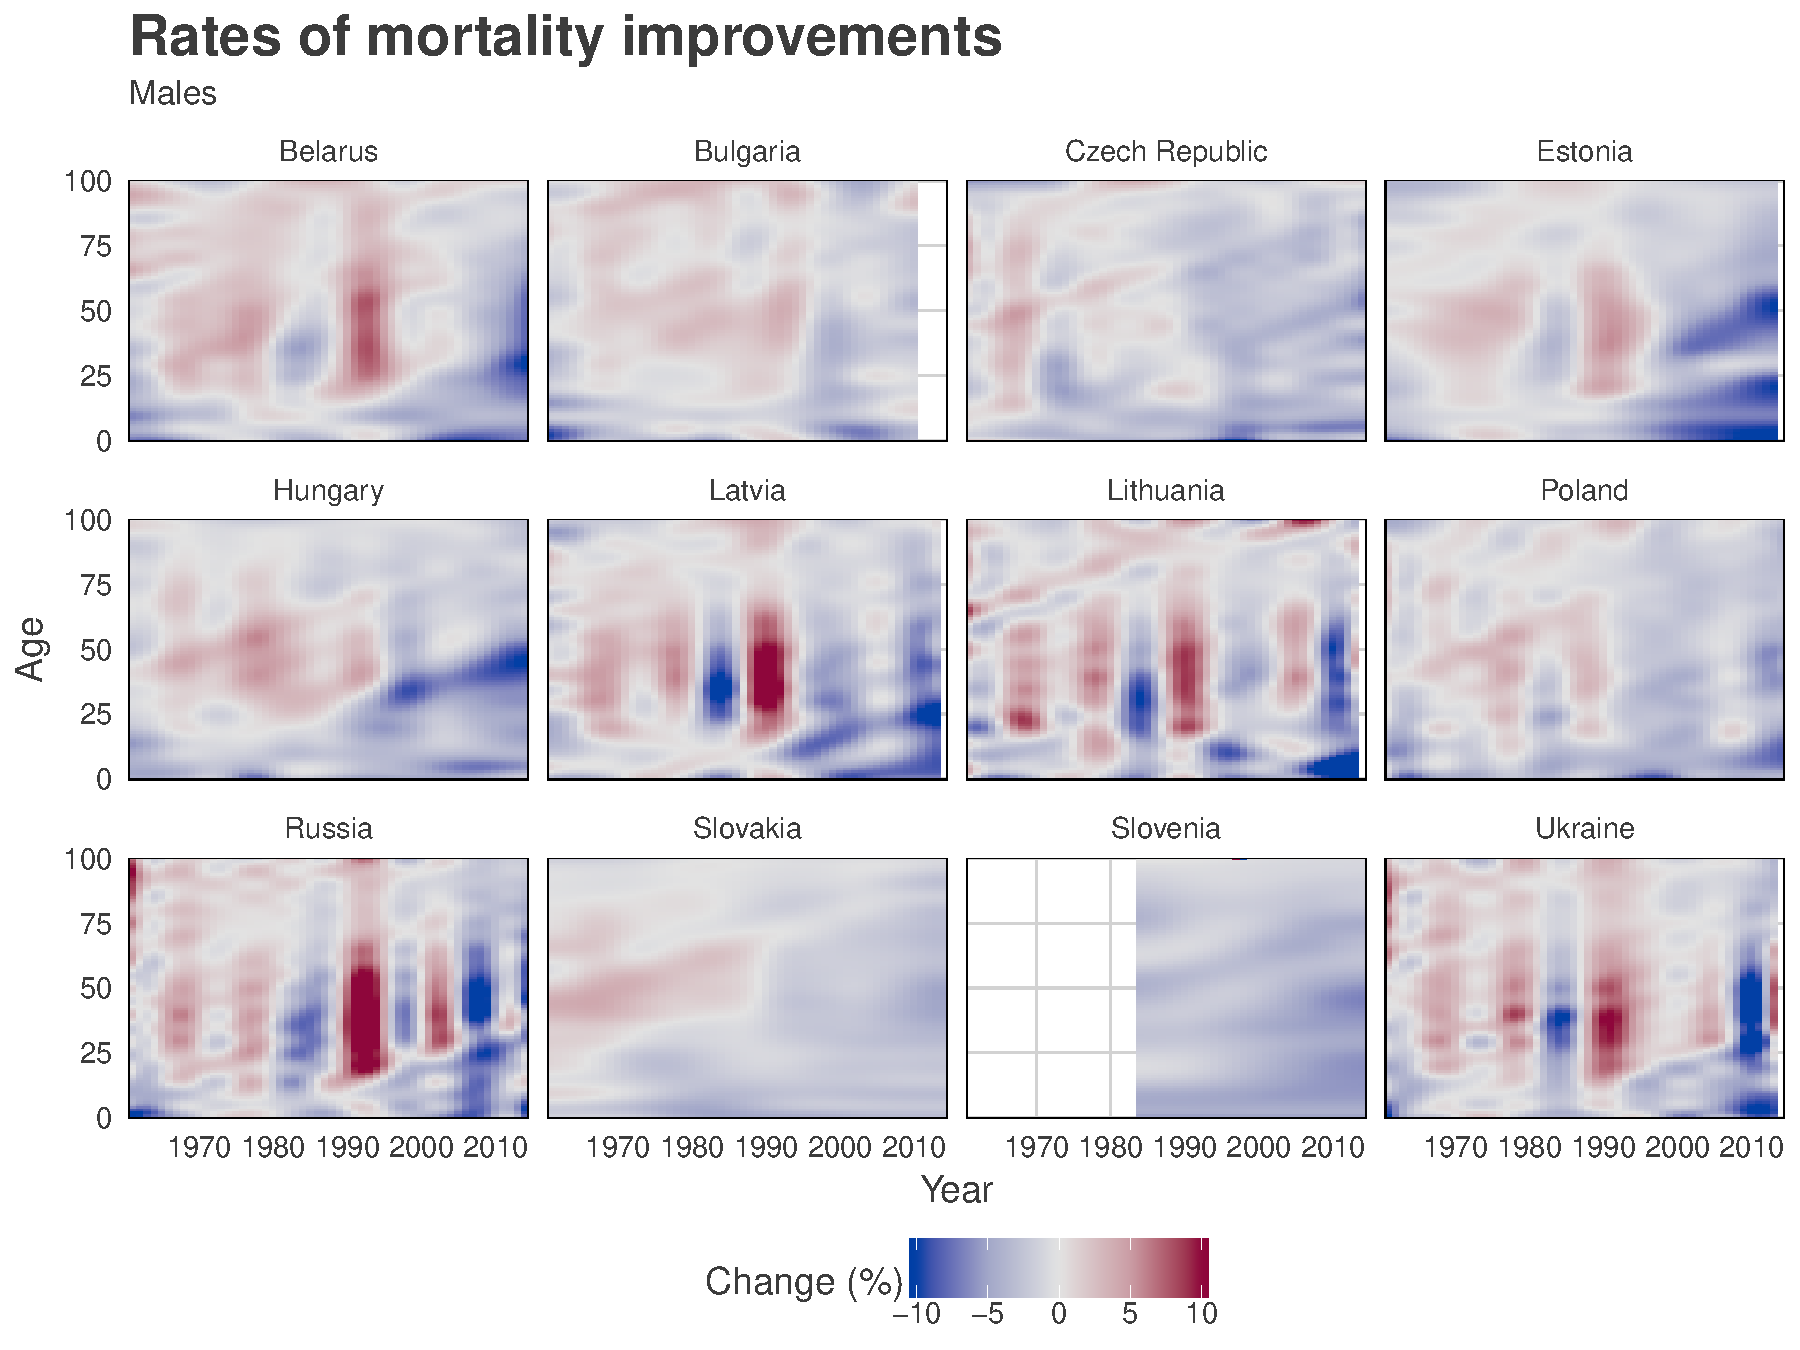
\includegraphics[scale=.55]{Figures/Romi_males.pdf}
\end{center}
Source: own calculations based on \citet{HMD} data. 
\begin{small}
Note: The regular light -grey areas indicate no data available.
\end{small}
\end{figure}

\begin{figure}[h!]
\centering
\caption{Trends in males life expectancy ($e_0$) and lifespan disparity  ($e^{\dagger}$) for 12 Eastern European countries, 1960-2014}
\label{Fig_LE&LD}
\begin{center}
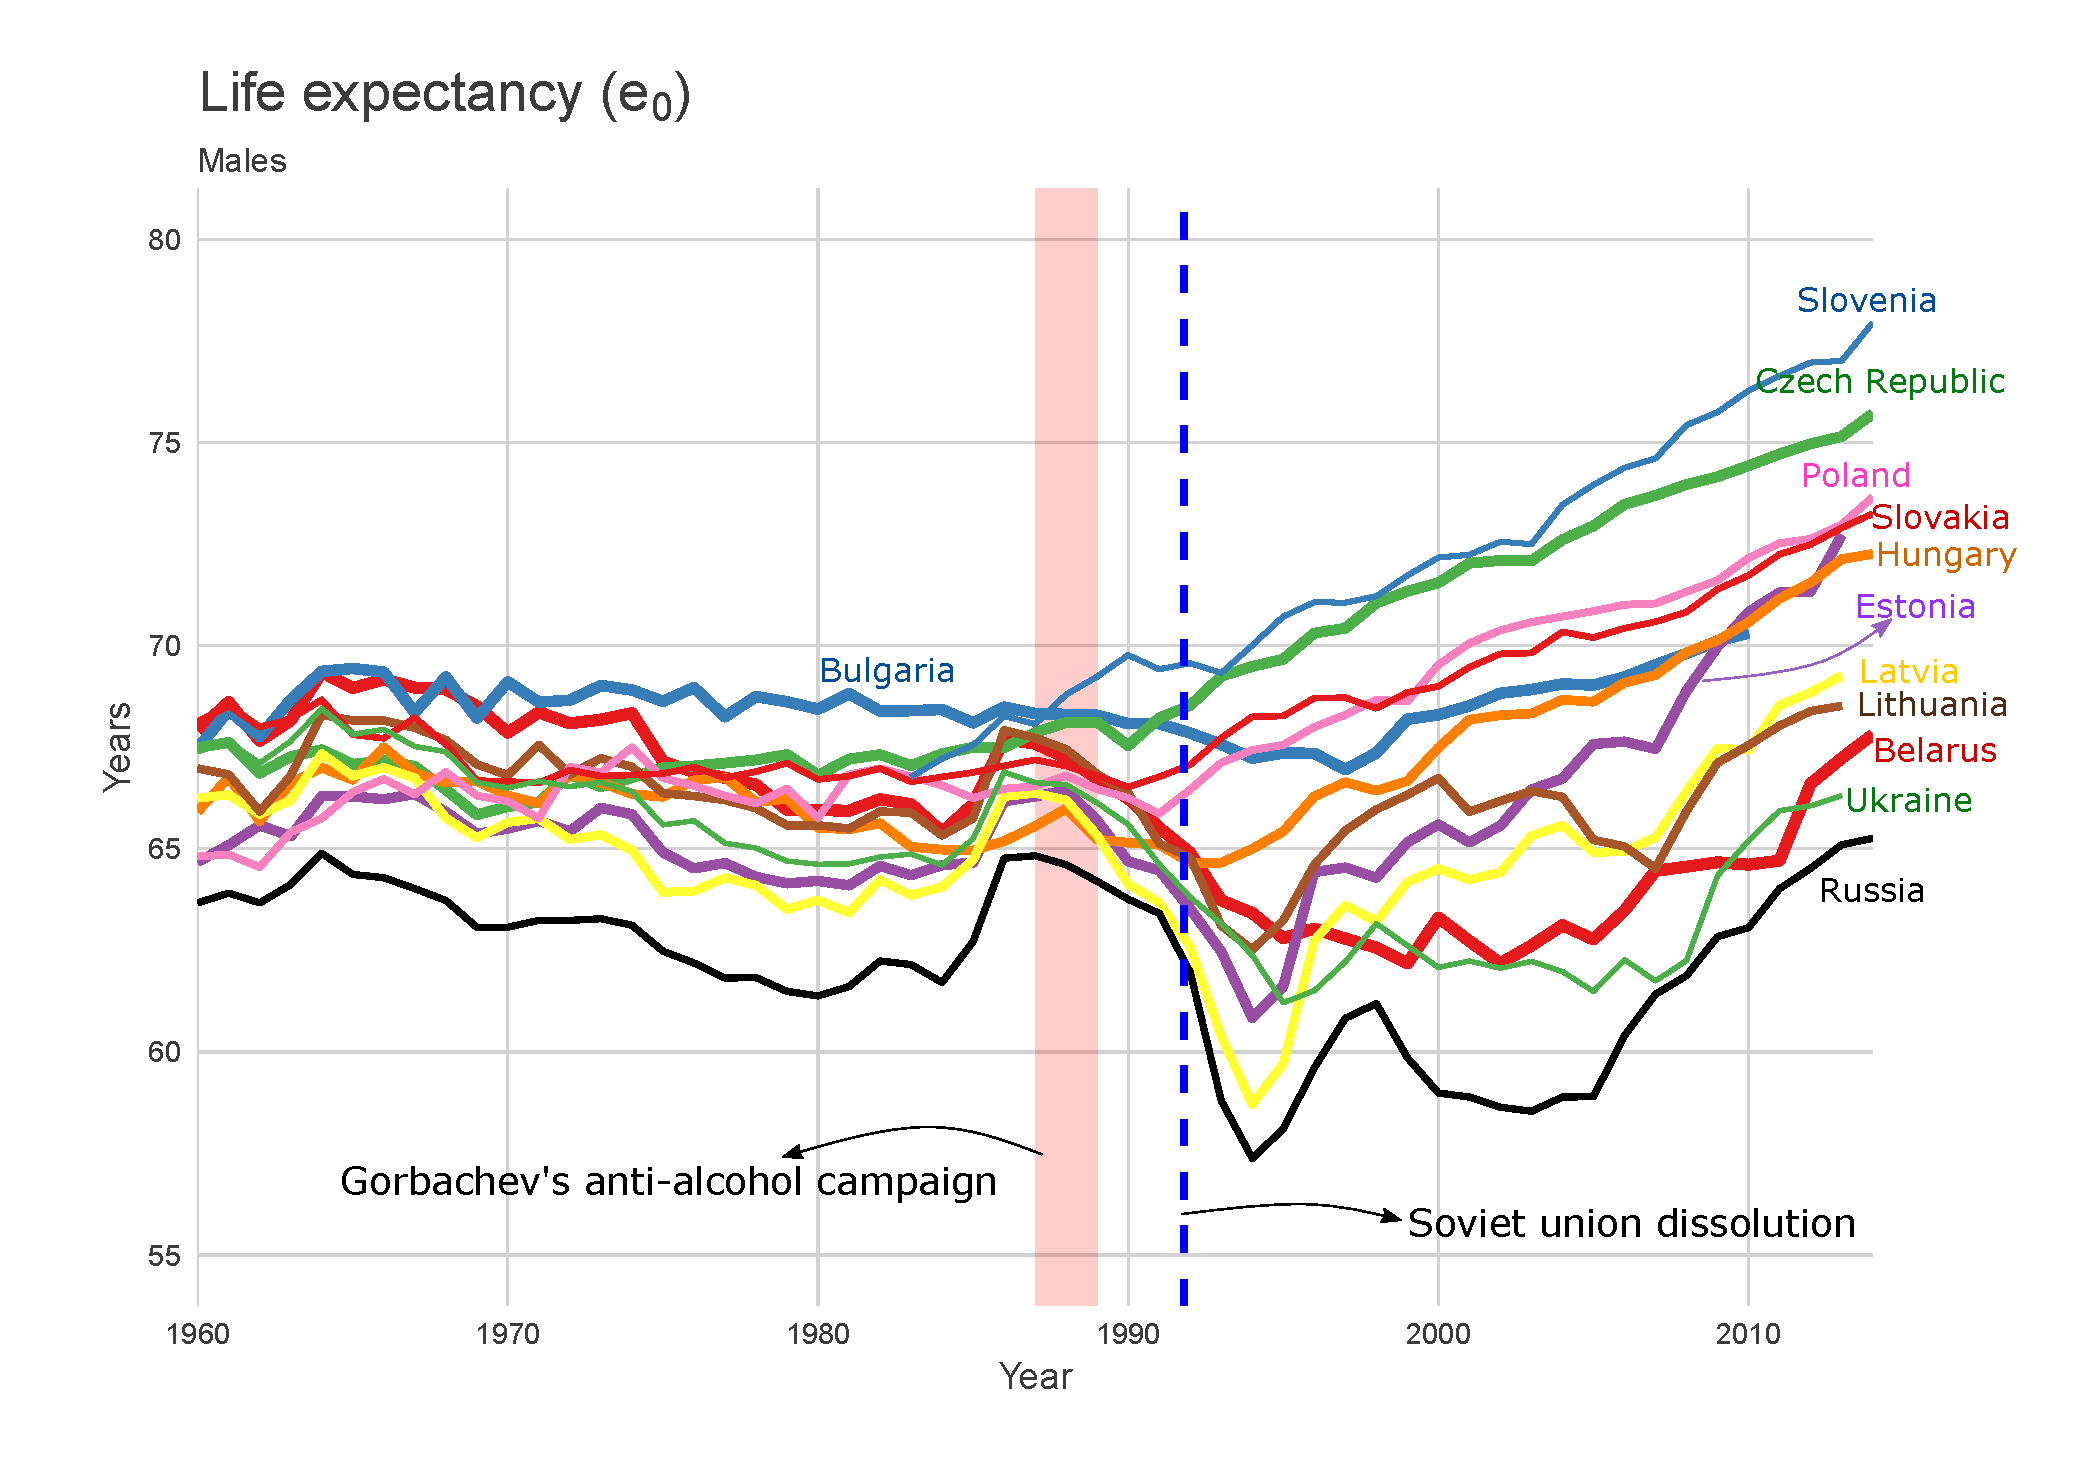
\includegraphics[scale=.40]{Figures/ex_males.pdf}
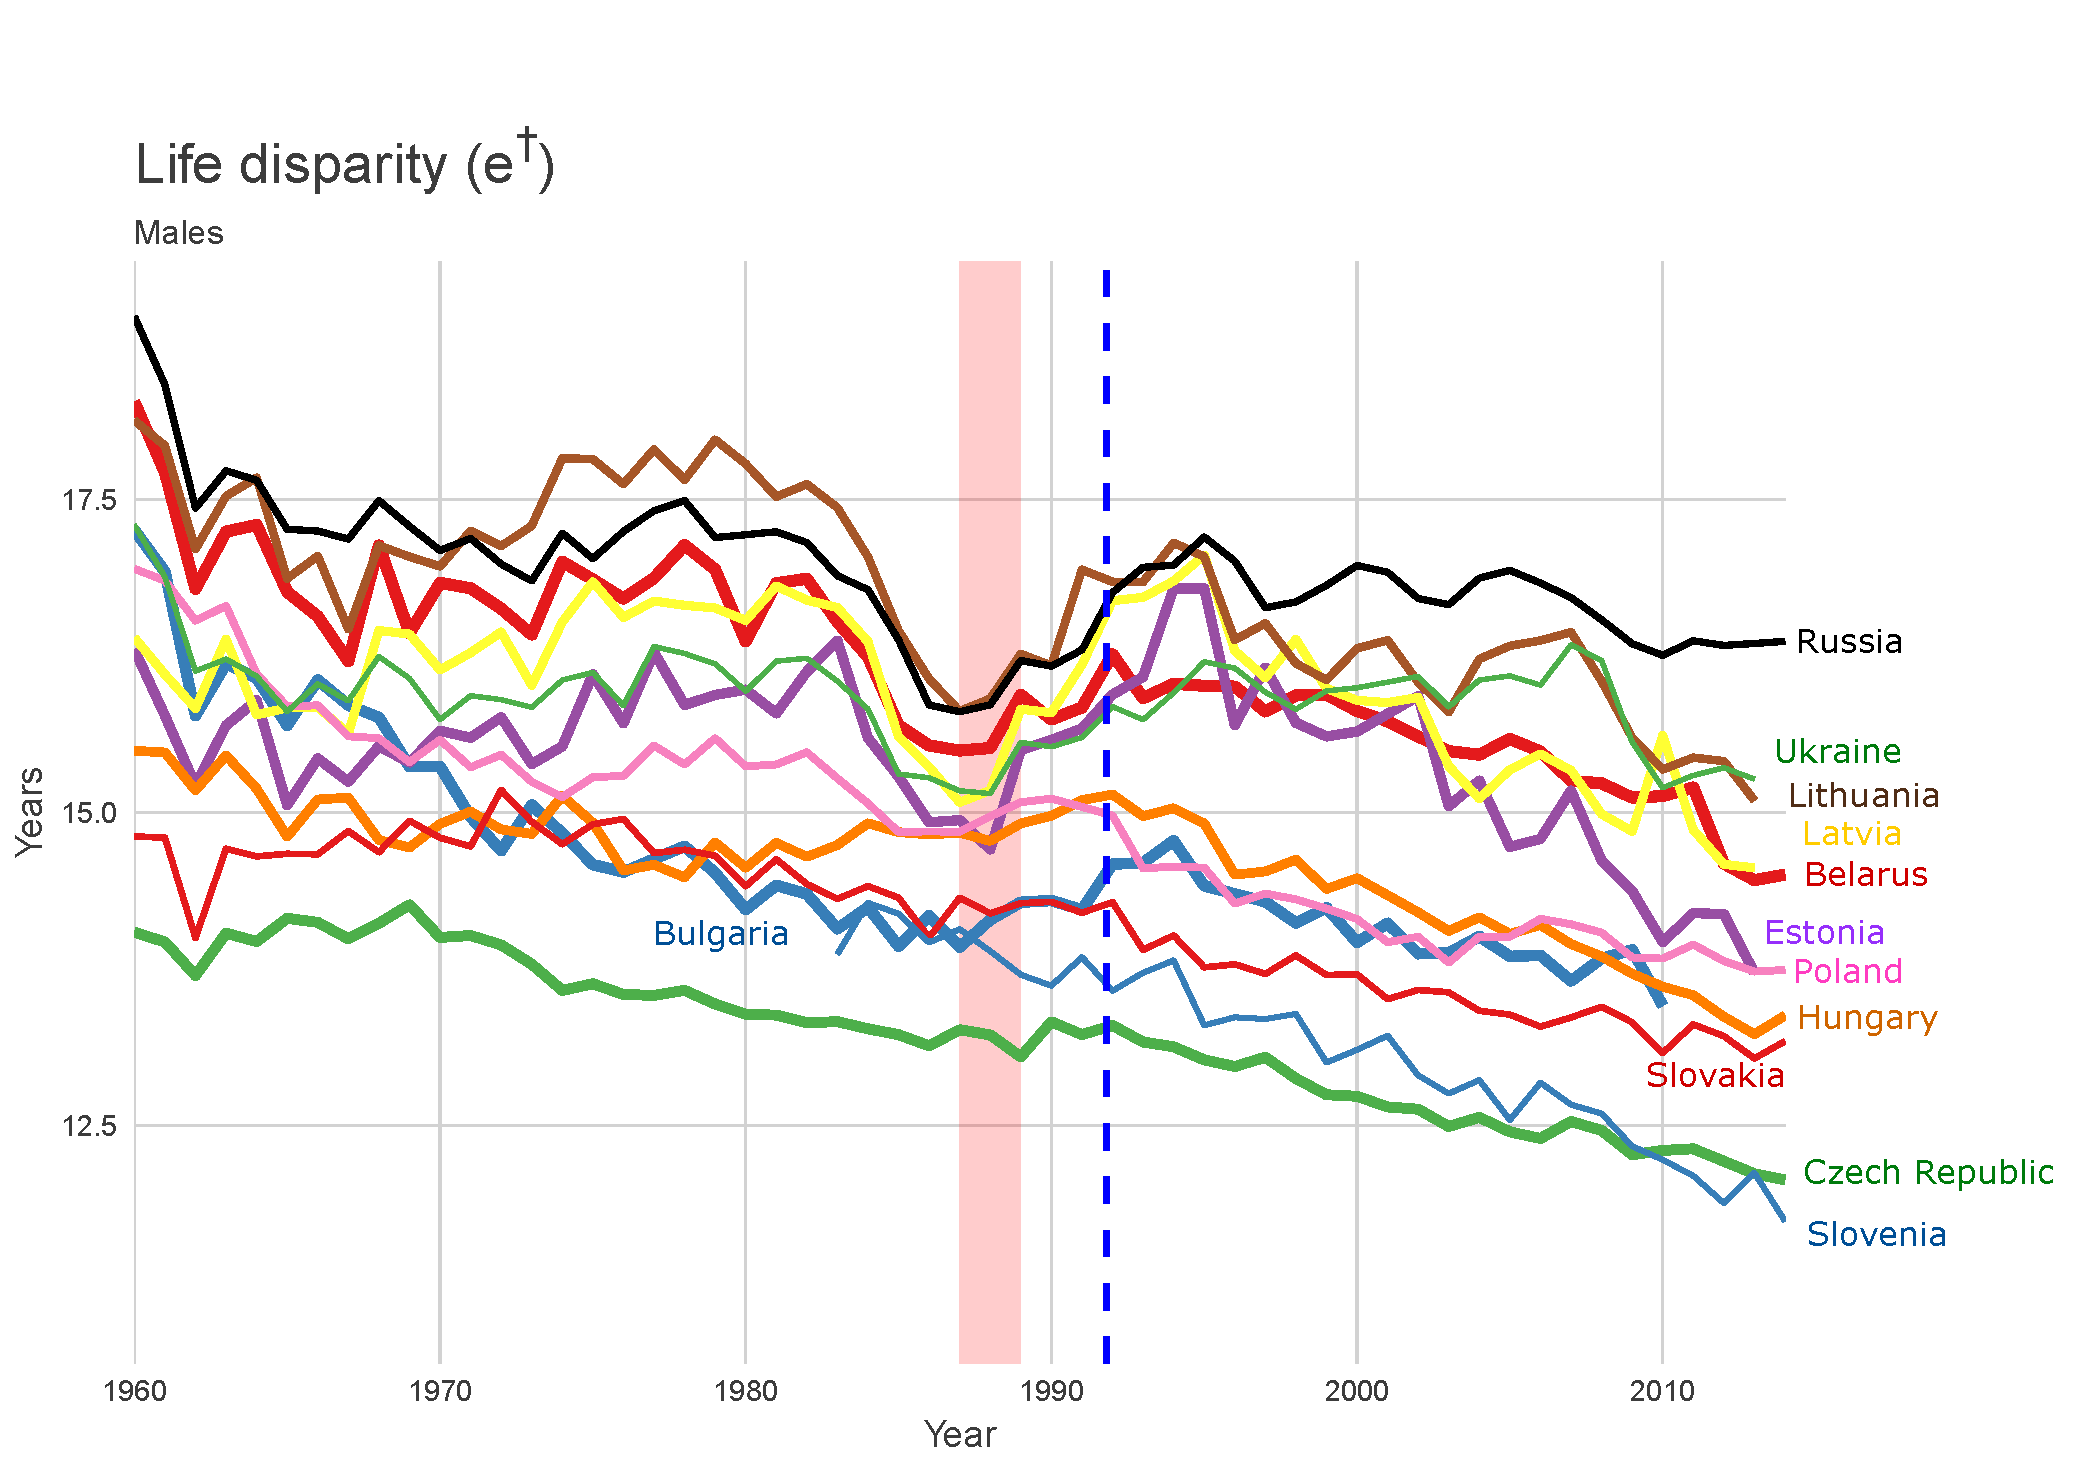
\includegraphics[scale=.40]{Figures/ed_males.pdf}
\end{center}
Source: own calculations based on \citet{HMD} data. 
\end{figure}

\newpage

\begin{figure}[h!]
\centering
\caption{Absolute and relative yearly changes in life expectancy and lifespan disparity, 1960-2010}
\label{Abs_changes}
\begin{center}
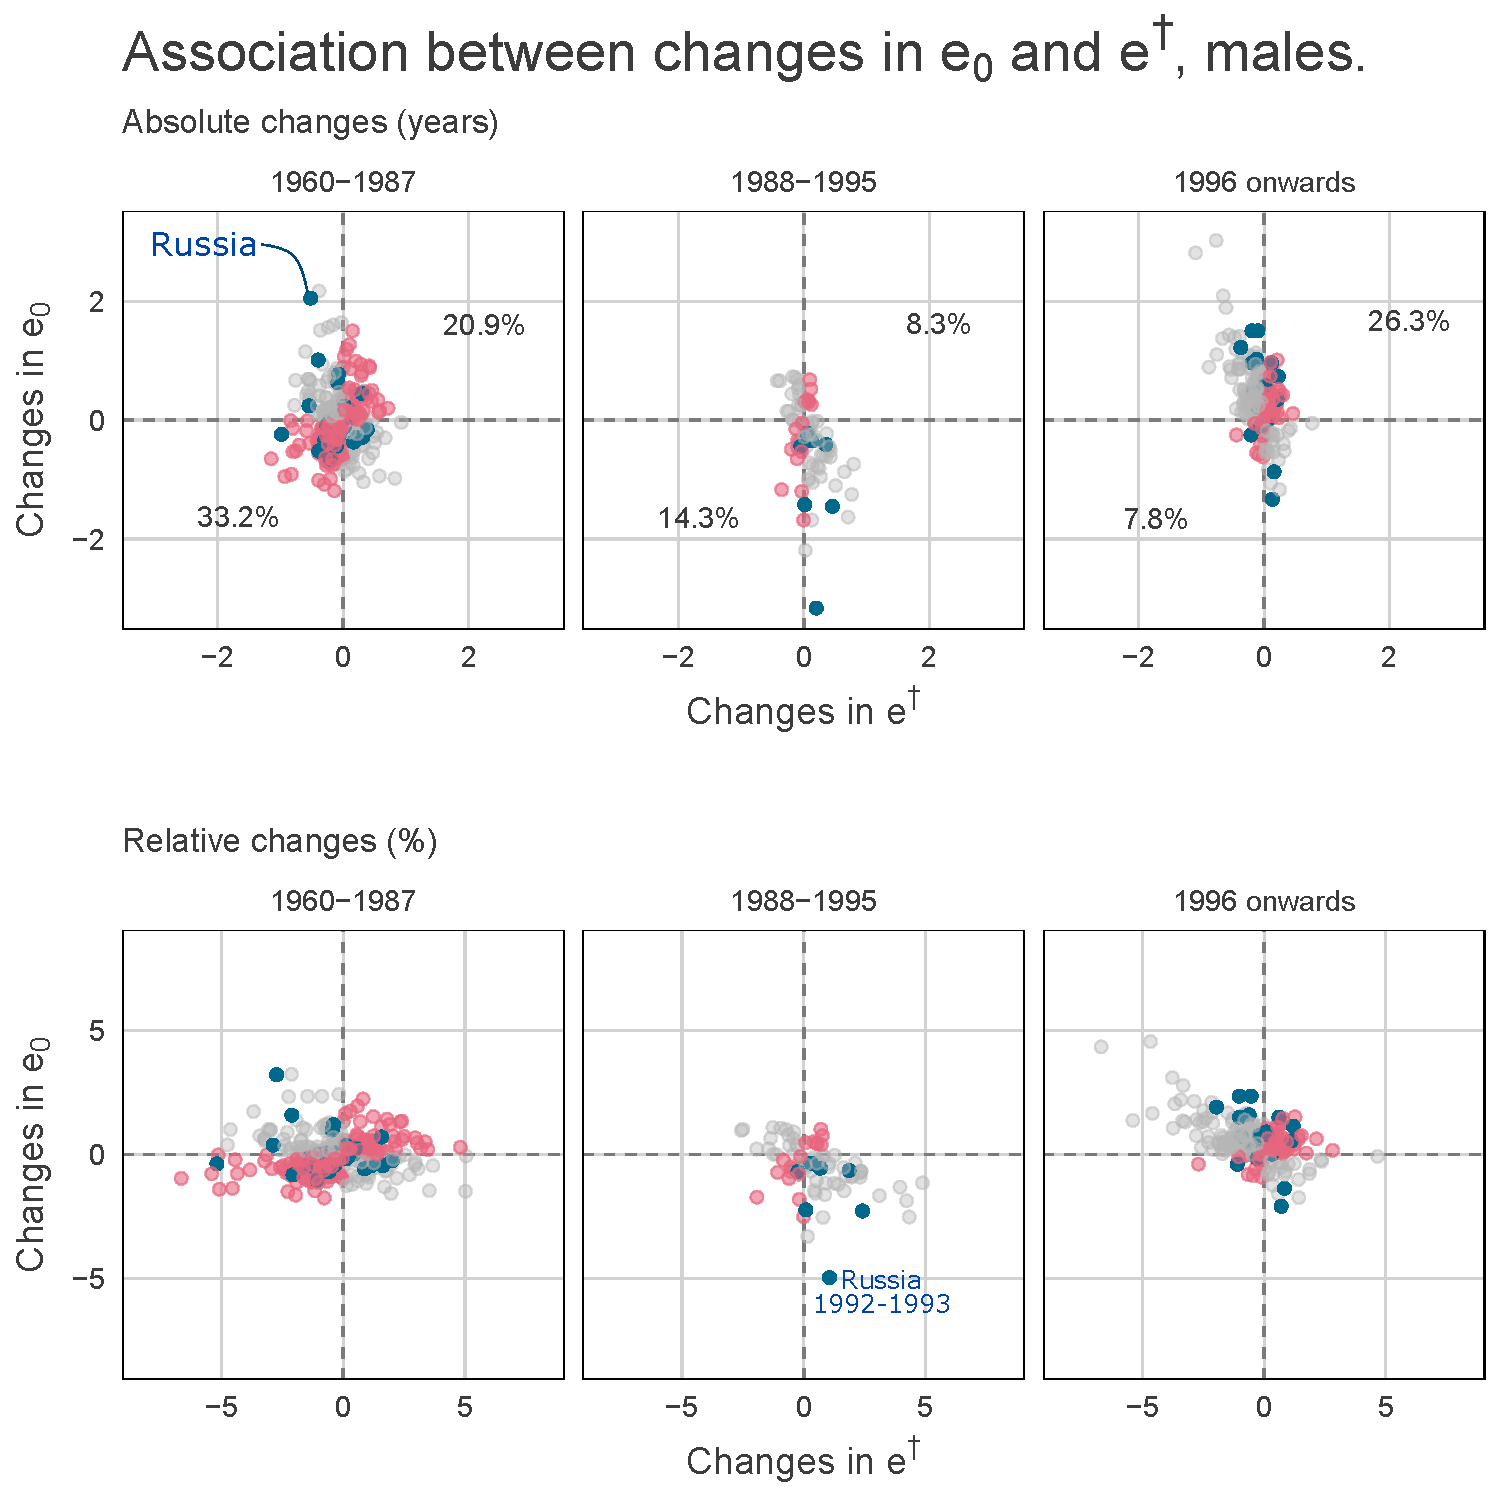
\includegraphics[scale=.65]{Figures/changes_males.pdf}
\end{center}
Source: own calculations based on \citet{HMD} data. Note: data for Slovenia begins in 1983. The black dots are related to changes experienced in Russia. The percentages correspond to the total changes occurred during each period.
\end{figure}

\newpage

\begin{figure}[h!]
\caption{Males' age-specific contributions to the change in lifespan disparity $e^\dagger$ by periods.}
\label{MalesDecomp}
\centering
\begin{center}
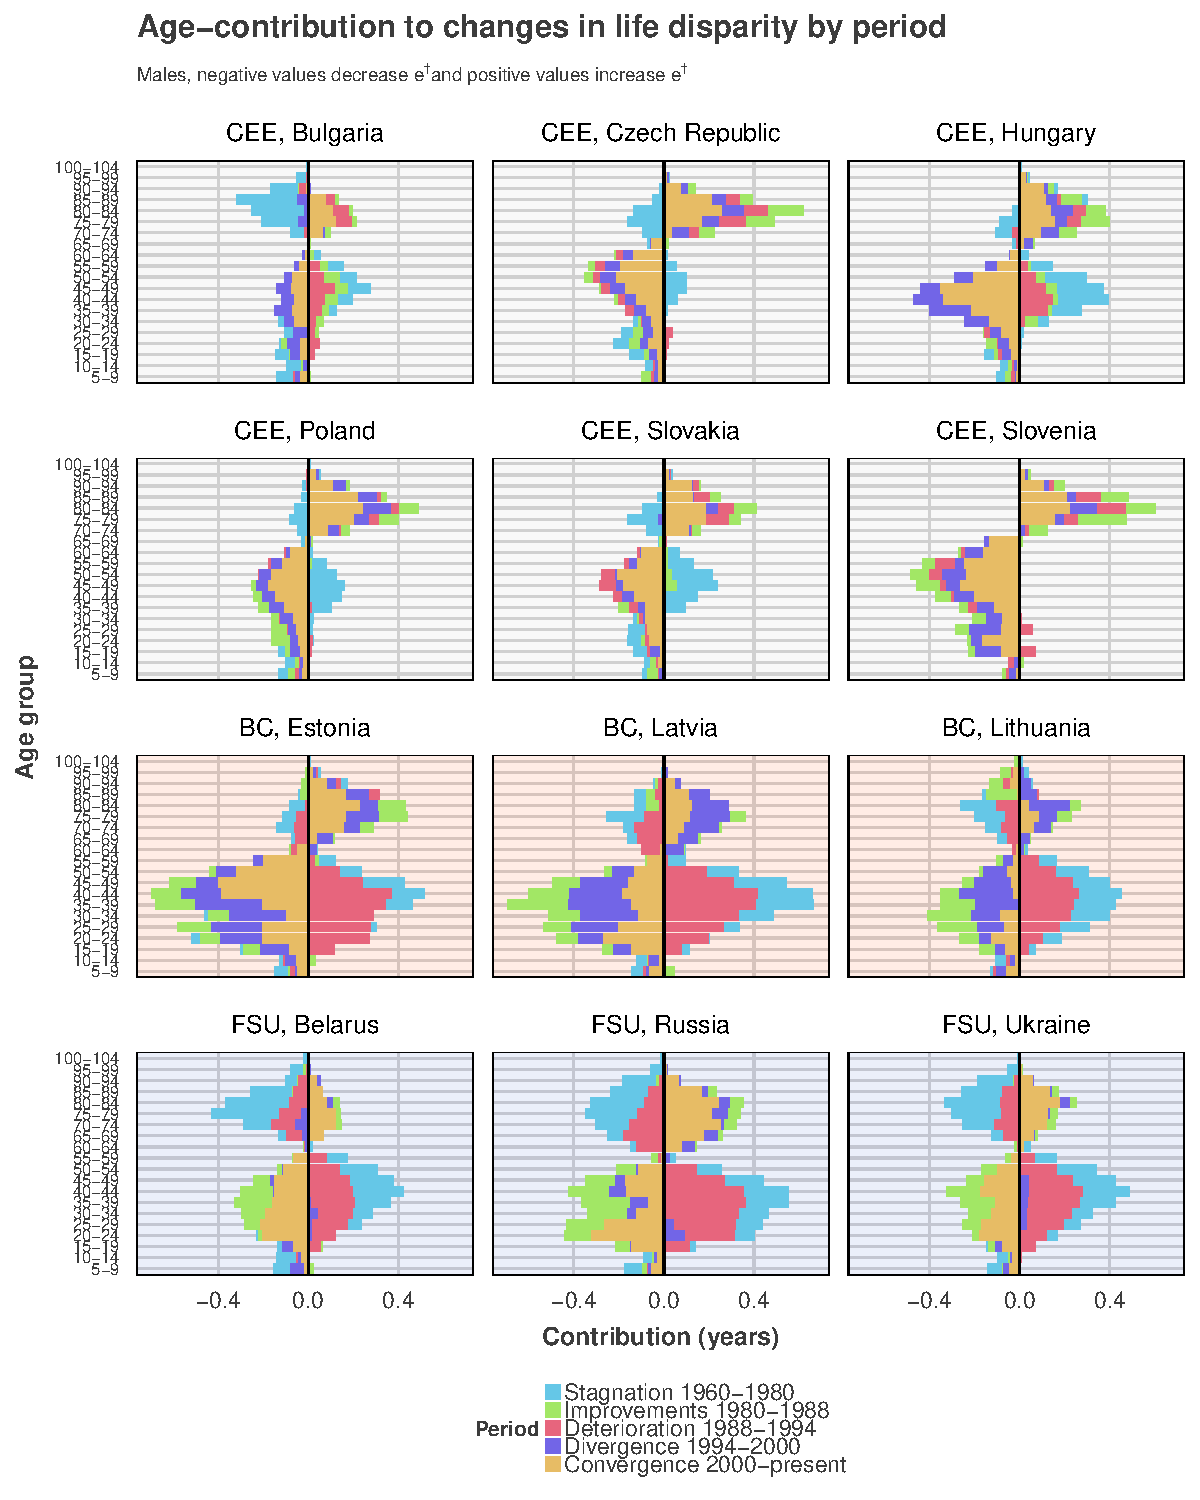
\includegraphics[scale=.52]{Figures/Age_ed_decomp_Males.pdf}
\end{center}
Source: own calculations based on \citet{HMD} data. Note: data for Slovenia begins in 1983.
\end{figure}

\newpage

\begin{figure}[h!]
\caption{Cause specific contributions to the change in  male lifespan disparity  $e^\dagger$, 1994-2000}
\label{Males_causes_1994}
\centering
\begin{center}
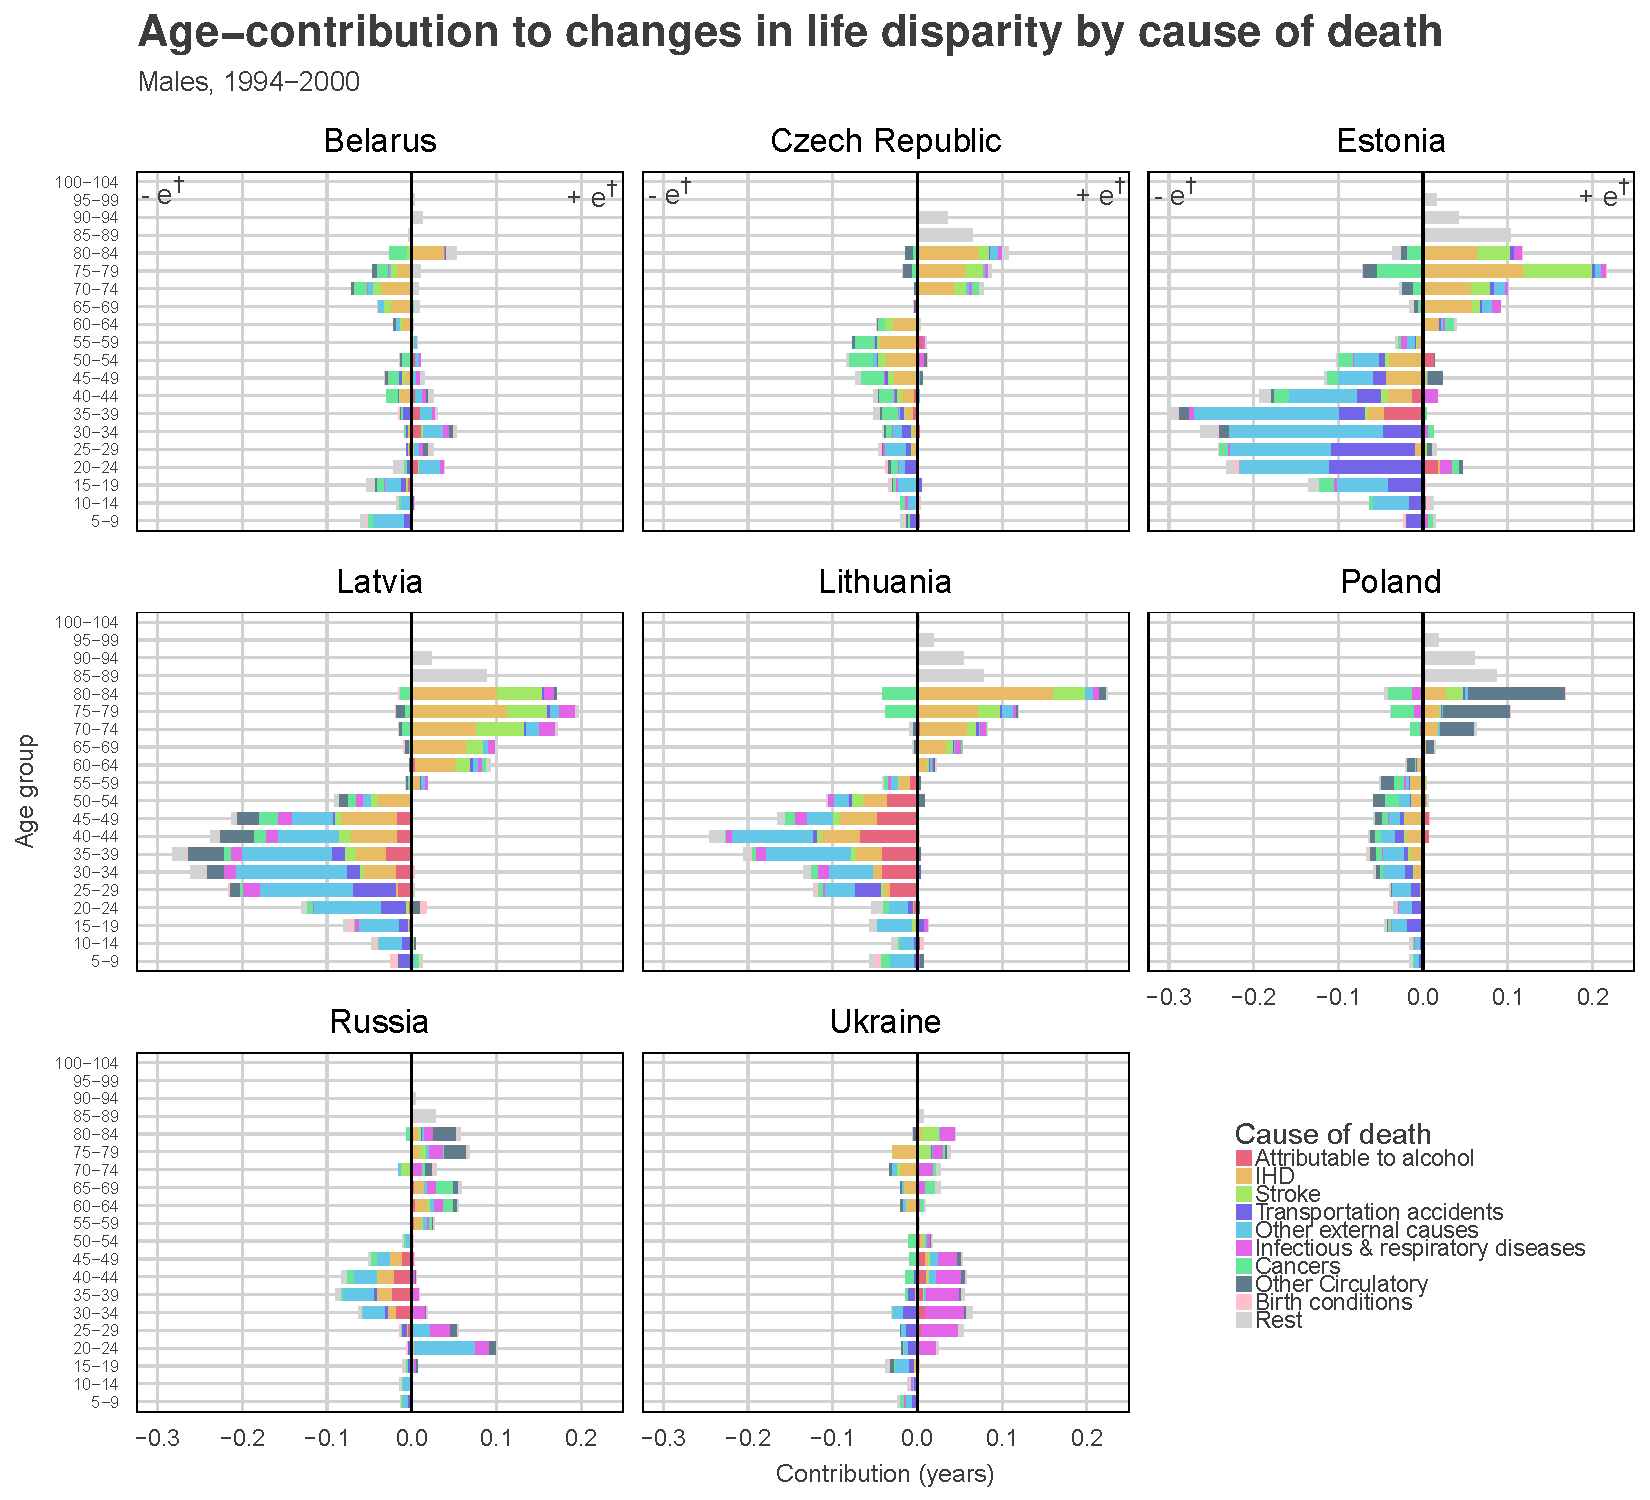
\includegraphics[scale=.53]{Figures/Cause_ed_decomp_Males_1.pdf}
\end{center}
Source: own calculations based on \citet{HcO} data. 
\end{figure}

\newpage

\begin{figure}[h!]
\caption{Cause specific contributions to the change in  male lifespan disparity  $e^\dagger$, 2000-2010}
\label{Males_causes_2000}
\centering
\begin{center}
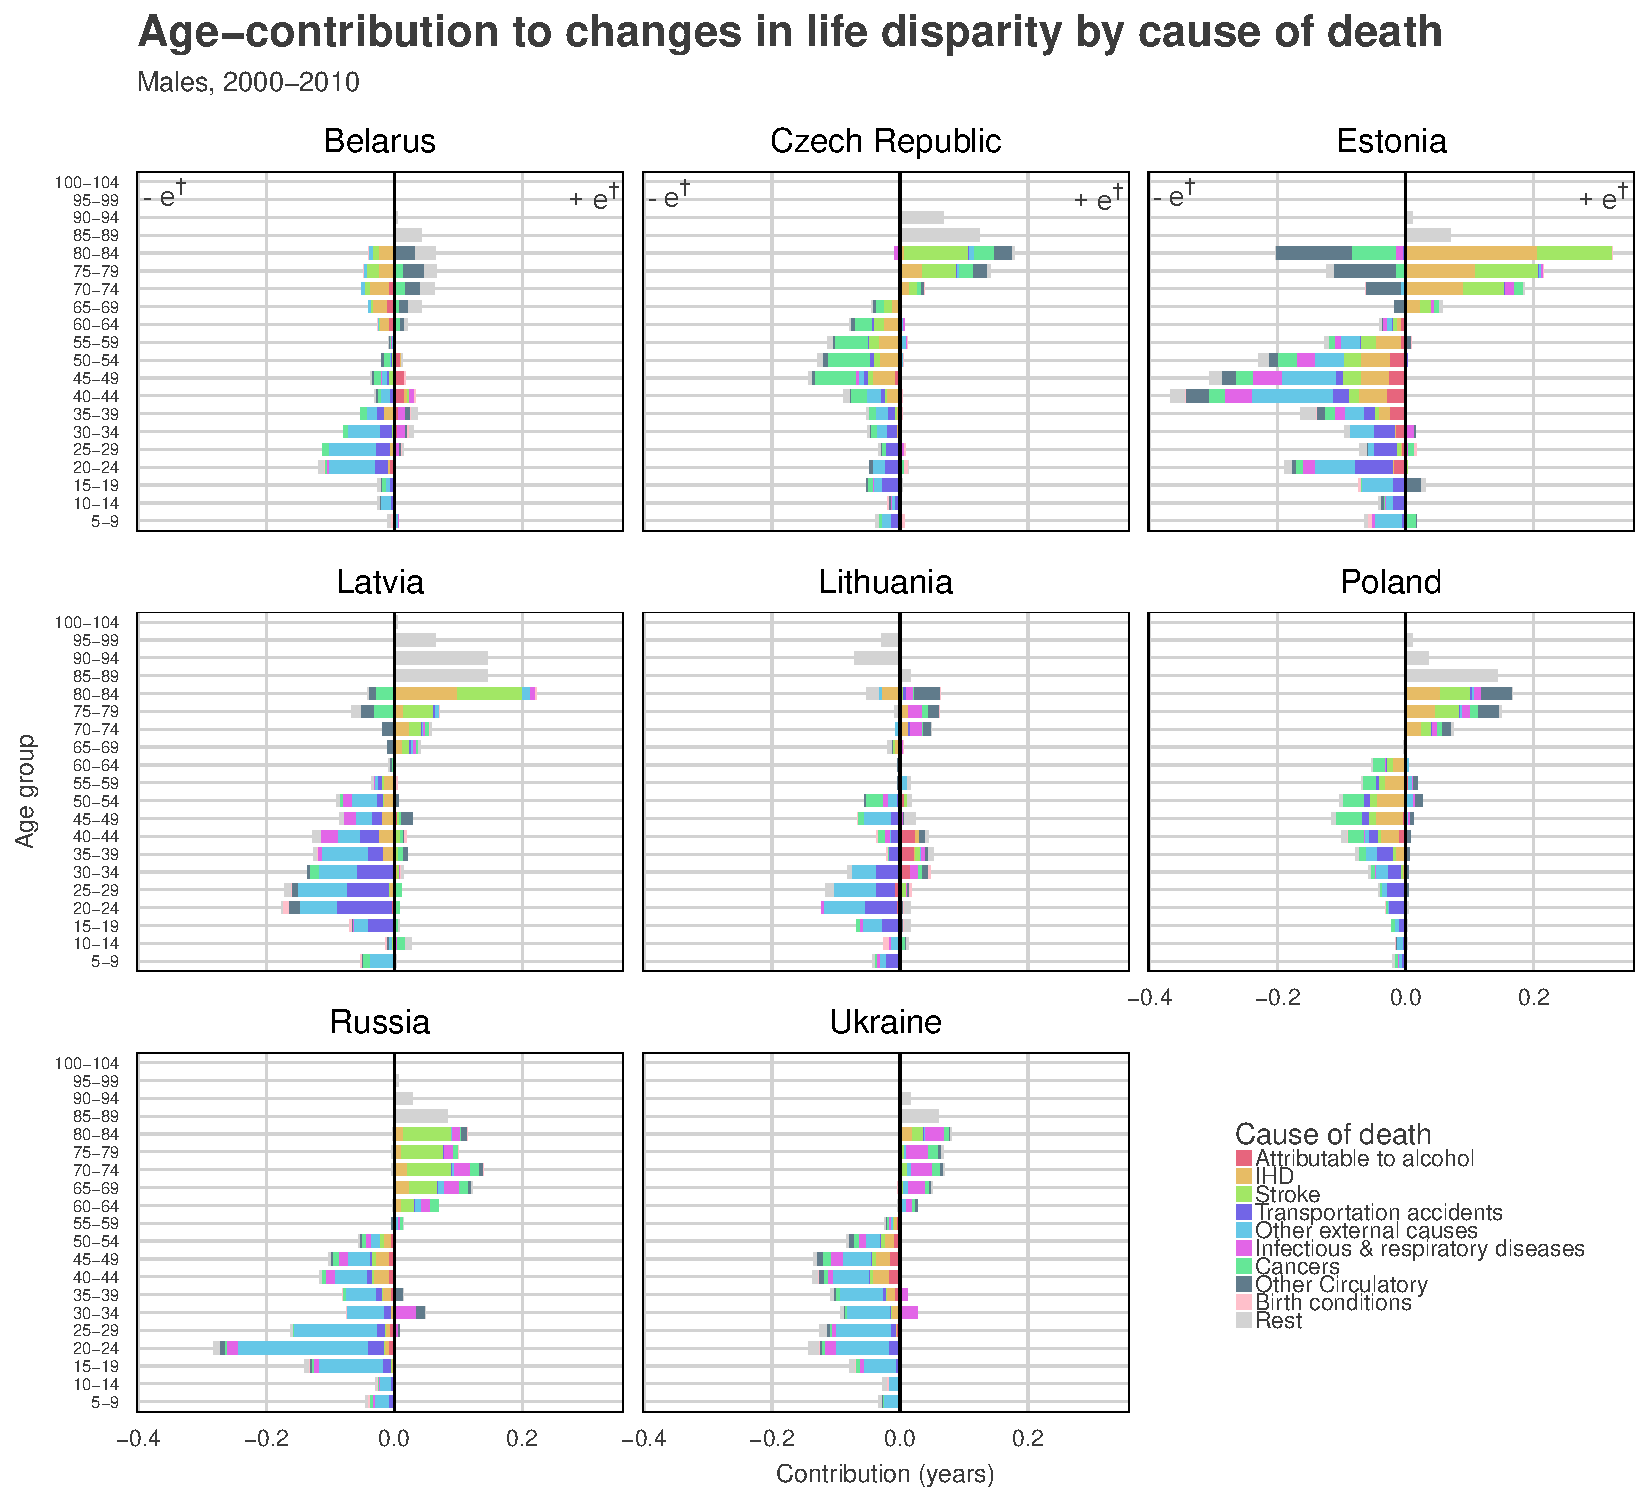
\includegraphics[scale=.53]{Figures/Cause_ed_decomp_Males_2.pdf}
\end{center}
Source: own calculations based on \citet{HcO} data. Note: data for Poland ends in 2009.
\end{figure}





%}
%\bibliographystyle{plainnat}


\end{document}
